\documentclass[a4paper,11pt,fleqn]{article}%fleqn pour aligner les equations à gauche
\usepackage{../../Styles/Eval}


\newcommand{\chnum}{Chapitre 17 et 4}
\newcommand{\chtitle}{DS2}
\newcommand{\dtype}{DS2}

\begin{document}
\maketitle
\textbf{Données pour toute l'évalution :}
\begin{itemize}
    \item Masse d'un proton : $m_p = \SI{1.6726E-27}{kg}$
    \item Masse d'un neutron : $m_n = \SI{1.6749E-27}{kg}$
    \item Masse d'un électron : $m_e = \SI{9,1084E-31}{kg}$
\end{itemize}
\section{Questionnaire}
\begin{enumerate}
    \item Ennoncer la loi des n\oe uds \vspace{2em}
    \begin{multicols}{2}
    \item Dans un circuit série les tensions aux bornes des dipoles :
        \begin{itemize}[label=$\square$]
            \item sont identiques
            \item sont égales à celle du générateur
            \item additionnées donnent celle du générateur
            \item sont nulles
        \end{itemize}
    \item La loi d'Ohm nous dit que :
        \begin{itemize}[label=$\square$]
            \item L'intensité est proportionnelle à la tension.
            \item La résistance d'un dipole est proportionnelle au courant qui la traverse.
            \item La tension est proportionnelle à l'intensité.
            \item La courbe de la résistance en fonction de la tension est une droite.
        \end{itemize}
    \item Par rapport à un atome, le noyau atomique est :
        \begin{itemize}[label=$\square$]
            \item Négligeable
            \item 100 000 fois plus grand
            \item 100 000 fois plus petit
            \item 100 000 fois moins massif
        \end{itemize}
    \item Indiquer les fausses informations :
        \begin{itemize}[label=$\square$]
            \item La masse d'un atome de chlore et d'un ion chlorure est environ la même.
            \item Il est possible de connaitre la position des électrons autour d'un noyau.
            \item Les éléments chimiques possèdent toujours le même nombre de neutrons dans le noyau.
            \item Un même élément chimique ne peut pas avoir des nombres de protons différents.
        \end{itemize}
    \item L'atome de chlore possède 17 protons et 20 neutrons. Sa masse sera donc de :
        \begin{itemize}[label=$\square$]
            \item \SI{6.184E-23}{kg}
            \item \SI{6.184E-26}{kg}
            \item \SI{6.193E-26}{kg}
            \item \SI{3.503E-26}{kg}
        \end{itemize}
    \item Dans une pastille de chlore, on retrouve \SI{4}{mg} de chlore. Cette pastille contient donc :
        \begin{itemize}[label=$\square$]
            \item \num{6.47E16} atomes de chlore
            \item \num{6.47E-16} atomes de chlore
            \item \num{6.46E19} atomes de chlore
            \item \num{6.46E-33} atomes de chlore
        \end{itemize}
    \item Sur le schéma suivant nommer chacune des mailles et chacun des n\oe uds.
        \begin{center}
            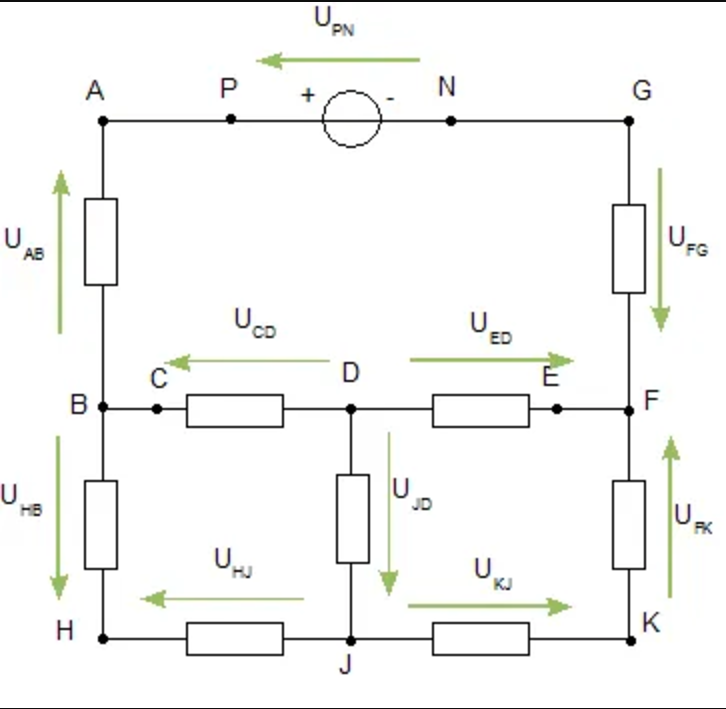
\includegraphics[width=.9\linewidth]{Resssources/2GT_DS2_24_Fig2.png}
        \end{center}
\end{multicols}
\end{enumerate}

\section{Electricité}
    On a relevé l'intensité parcourant un dipôle pour les tensiosn variables.\\

\begin{tabular}{|c|c|c|c|c|c|c|c|c|c|}
    \hline
    \textbf{U (V)} & \num{0} & \num{0.67} & \num{1.27} &\num{2.03} &\num{2.73} &\num{3.49} &\num{4.21} &\num{4.94}\\ 
    \hline
    \textbf{I (mA)} & \num{0} & \num{3.0} & \num{5.7} &\num{9.1} &\num{12.3} &\num{15.7} &\num{19.0} &\num{22.3} \\
    \hline
\end{tabular}
\begin{enumerate}[resume]
    \item Représenter le nuage de points $U = f(I)$ (attention aux unités !).
    \item Tracer la droite moyenne de cette courbe.
    \item Calculer la pente de la courbe.
    \item En déduire la valeur de la résistance étudiée.
\end{enumerate}

\section{L'iode en tant qu'oligoélément}
L'iode est un élément chimique indispensable au fonctionnementy de notre organisme. Même en très faible quantioté, il permet la synthèse d'hotmones thyroïdiennes. La dose conseillée d'iode que doit apporter l'aimentation est $m = \SI{150}{\micro\gram}$ par jour pour des adolescents.\\
\textbf{Données :}
\begin{itemize}
    \item Ecriture conventionnelle d'un noyaud d'iode : $^{127}_{53}I$
    \item conversion : \SI{1}{\micro\gram} correspond à \SI{1E-6}{\gram}
\end{itemize}
\begin{enumerate}
    \item Etablir la composition d'un noyau d'iode.
    \item Exprimer puis calculer la masse d'un atome d'iode.
    \item Exprimer puis calculer le nombre $N$ d'atomes d'iode qu'un adolescent doit consommer chaque jour. Conclure.
\end{enumerate}
\end{document}


\subsection*{Partie 1}
\begin{figure}[h!]
    \begin{minipage}{.48\linewidth}
        \begin{circuitikz}
            \draw(0,0) node[below]{A} to [short,o-,i=$I$] ++ (1,0)
            to [short] ++ (0,1)
            to [R,l_=$R_2$,i>^=$I_2$] ++(2,0)
            to [R,l_=$R_3$] ++(2,0)
            to [short] ++ (0,-2)
            to [R,l_=$R_1$,i^<=$I_1$] ++ (-4,0)
            to [short] ++(0,1);
            \draw(6,0) node[below]{B} to [short,o-] ++(-1,0);
            \draw[-Stealth] (6,-2) to (0,-2);
            \draw(3,-2) node[above]{$U_{AB}$};
        \end{circuitikz}\\
    \end{minipage}\hspace{.02\linewidth}
    \begin{minipage}{.48\linewidth}
        \textbf{Données :}
        \begin{itemize}
            \item $R_1 = \SI{10}{\ohm}$
            \item $R_2 = \SI{5.0}{\ohm}$
            \item $R_3 = \SI{3.0}{\ohm}$
            \item $U_{AB} = \SI{10}{\volt}$
        \end{itemize}
    \end{minipage}
\end{figure}
\begin{enumerate}
    \item Quelle est l'intensité $I_1$ du courant traversant $R_1$ ?
    \item Quelle est l'intensité $I_2$ du courant traversant $R_2$ et $R_3$ ?
    \item Calculer la valeur de l'intensité $I$ du courant dans la branche principale. En déduire la valeur de la résistance globale du circuit que l'on notera $R$.
\end{enumerate}

\subsection*{Partie 2}
